\documentclass[11pt,oneside,openany]{book}

% ============================================================================
% PACKAGES & TYPOGRAPHY
% ============================================================================
\usepackage[utf8]{inputenc}
\usepackage[T1]{fontenc}
\usepackage{mathpazo} % Palatino serif for elegant book body text
\usepackage[scaled=0.88]{helvet} % Helvetica sans-serif for headings & UI labels
\usepackage{courier}
\usepackage{microtype}
\usepackage[
  paperwidth=6.5in,
  paperheight=9.5in,
  top=0.95in,
  bottom=0.95in,
  left=0.85in,
  right=0.85in,
  headheight=24pt
]{geometry}
\emergencystretch=1.5em

\usepackage{graphicx}
\usepackage{xcolor}
\usepackage{tikz}
\usetikzlibrary{calc,positioning,shapes.geometric,arrows.meta}
\usepackage{tcolorbox}
\tcbuselibrary{skins,breakable}
\usepackage{amsmath,amssymb}
\usepackage{booktabs}
\usepackage{tabularx}
\usepackage{enumitem}
\usepackage{fancyhdr}
\usepackage{titlesec}
\usepackage{hyperref}

% Map Romanian characters cleanly for pdflatex T1
\DeclareUnicodeCharacter{0219}{\textcommabelow{s}}
\DeclareUnicodeCharacter{0218}{\textcommabelow{S}}
\DeclareUnicodeCharacter{021B}{\textcommabelow{t}}
\DeclareUnicodeCharacter{021A}{\textcommabelow{T}}
\DeclareUnicodeCharacter{0103}{\u{a}}
\DeclareUnicodeCharacter{0102}{\u{A}}
\DeclareUnicodeCharacter{00EE}{\^{i}}
\DeclareUnicodeCharacter{00CE}{\^{I}}
\DeclareUnicodeCharacter{00E2}{\^{a}}
\DeclareUnicodeCharacter{00C2}{\^{A}}

% ============================================================================
% COLOR PALETTE (Matching Aetherium's Celestial Sanctuary Theme)
% ============================================================================
\definecolor{CosmicBg}{HTML}{05070D}
\definecolor{CosmicPanel}{HTML}{0B101E}
\definecolor{CosmicDeep}{HTML}{0F172A}
\definecolor{AetherCyan}{HTML}{22D3EE}
\definecolor{AetherCyanDark}{HTML}{0E7490}
\definecolor{AetherIndigo}{HTML}{4F46E5}
\definecolor{AetherIndigoLight}{HTML}{818CF8}
\definecolor{AetherEmerald}{HTML}{10B981}
\definecolor{AetherEmeraldDark}{HTML}{047857}
\definecolor{AetherAmber}{HTML}{F59E0B}
\definecolor{AetherAmberDark}{HTML}{B45309}
\definecolor{SlateText}{HTML}{1E293B}
\definecolor{SlateMuted}{HTML}{64748B}
\definecolor{BoxBg}{HTML}{F8FAFC}
\definecolor{BoxBorder}{HTML}{CBD5E1}

% ============================================================================
% HYPERREF SETUP
% ============================================================================
\hypersetup{
  colorlinks=true,
  linkcolor=AetherIndigo,
  urlcolor=AetherCyanDark,
  citecolor=AetherEmeraldDark,
  pdftitle={Aetherium: Where Celestial Physics Meets Receptive Music Therapy},
  pdfauthor={Dragos Iorgulescu (Voidwave Lab)},
  pdfsubject={Generative Ambient Soundscape & Receptive Music Therapy Sanctuary},
  pdfkeywords={Aetherium, Generative Music, Receptive Music Therapy, Anxiety Regulation, ISO Principle, Polyvagal Theory, EMDR, Voidwave Lab, Dragos Iorgulescu}
}

% ============================================================================
% HEADERS, FOOTERS & PAGE NUMBERING
% ============================================================================
\pagestyle{fancy}
\fancyhf{}
\fancyhead[L]{\sffamily\footnotesize\color{SlateMuted}\textsc{Aetherium} $\cdot$ \leftmark}
\fancyhead[R]{\sffamily\footnotesize\color{SlateMuted}\textsc{Voidwave Lab}}
\fancyfoot[C]{\sffamily\small\color{SlateText}\textbf{\thepage}}
\renewcommand{\headrulewidth}{0.4pt}
\renewcommand{\headrule}{\hbox to\headwidth{\color{BoxBorder}\leaders\hrule height \headrulewidth\hfill}}
\renewcommand{\footrulewidth}{0pt}

\fancypagestyle{plain}{
  \fancyhf{}
  \fancyfoot[C]{\sffamily\small\color{SlateText}\textbf{\thepage}}
  \renewcommand{\headrulewidth}{0pt}
}

% ============================================================================
% CHAPTER & SECTION STYLING
% ============================================================================
\titleformat{\chapter}[display]
  {\normalfont\sffamily}
  {\tikz[baseline=(char.base)]{
    \node[fill=CosmicDeep, text=AetherCyan, rounded corners=4pt, inner xsep=10pt, inner ysep=5pt, font=\sffamily\bfseries\footnotesize\scshape] (char) {CHAPTER \thechapter};
  }}
  {10pt}
  {\huge\bfseries\color{CosmicDeep}}
  [\vspace{6pt}{\color{AetherCyanDark}\titlerule[1.2pt]}]

\titleformat{\section}
  {\normalfont\sffamily\Large\bfseries\color{CosmicDeep}}
  {\color{AetherCyanDark}\thesection}
  {0.6em}
  {}

\titleformat{\subsection}
  {\normalfont\sffamily\large\bfseries\color{SlateText}}
  {\color{AetherIndigo}\thesubsection}
  {0.6em}
  {}

% ============================================================================
% CALLOUT BOXES
% ============================================================================
\newtcolorbox{sanctuarybox}[2][]{
  enhanced,
  breakable,
  colback=BoxBg,
  colframe=AetherCyanDark,
  colbacktitle=CosmicDeep,
  coltitle=white,
  fonttitle=\sffamily\bfseries\small,
  title={#2},
  arc=5pt,
  boxrule=0.8pt,
  left=10pt,
  right=10pt,
  top=8pt,
  bottom=8pt,
  #1
}

\newtcolorbox{clinicalbox}[2][]{
  enhanced,
  breakable,
  colback=BoxBg,
  colframe=AetherEmeraldDark,
  colbacktitle=AetherEmeraldDark,
  coltitle=white,
  fonttitle=\sffamily\bfseries\small,
  title={#2},
  arc=5pt,
  boxrule=0.8pt,
  left=10pt,
  right=10pt,
  top=8pt,
  bottom=8pt,
  #1
}

\setlength{\parskip}{0.45em}
\setlength{\parindent}{0pt}
\setlist[itemize]{topsep=4pt, itemsep=3pt, leftmargin=1.5em}
\setlist[enumerate]{topsep=4pt, itemsep=4pt, leftmargin=1.6em}

\begin{document}

% ============================================================================
% FULL-BLEED EBOOK COVER PAGE
% ============================================================================
\begin{titlepage}
\thispagestyle{empty}
\begin{tikzpicture}[remember picture, overlay]
  % 1. Full-page deep cosmic background matching the logo's dark space
  \fill[CosmicBg] (current page.south west) rectangle (current page.north east);

  % 2. Subtle ambient celestial rings & Meridian axis behind the cover art
  \draw[AetherIndigo!30!CosmicBg, line width=0.6pt]
    ([yshift=-0.3in]current page.center) circle (2.65in);
  \draw[AetherCyan!22!CosmicBg, line width=0.5pt, dashed]
    ([yshift=-0.3in]current page.center) circle (2.95in);
  \draw[AetherCyan!35!CosmicBg, line width=0.7pt]
    ([yshift=2.8in]current page.center) -- ([yshift=-2.8in]current page.center);

  % 3. Top Organization Badge
  \node[
    anchor=north,
    yshift=-0.65in,
    font=\sffamily\footnotesize\bfseries,
    text=AetherCyan
  ] at (current page.north) {VOIDWAVE LAB $\cdot$ OPEN-SOURCE PSYCHOACOUSTIC SANCTUARY};

  % 4. Book Title (Software Name)
  \node[
    anchor=north,
    yshift=-1.0in,
    font=\sffamily\fontsize{36}{40}\selectfont\bfseries,
    text=white
  ] at (current page.north) {A E T H E R I U M};

  % 5. Attention-Grabbing Subtitle
  \node[
    anchor=north,
    yshift=-1.62in,
    font=\normalfont\itshape\fontsize{14.5}{19}\selectfont,
    text=AetherCyan!85!white,
    align=center,
    text width=5.2in
  ] at (current page.north) {Where Celestial Physics Meets Receptive Music Therapy};

  \node[
    anchor=north,
    yshift=-1.98in,
    font=\sffamily\fontsize{9.5}{13}\selectfont,
    text=white!75!AetherIndigoLight,
    align=center,
    text width=5.0in
  ] at (current page.north) {Turn Orbiting Light into Living Soundscapes for Anxiety Relief,\\Mood Regulation, and Clinical Practice};

  % 6. Scaled Program Logo (Clipped inside a circular cosmic halo so corners blend seamlessly)
  \begin{scope}[shift={([yshift=-0.35in]current page.center)}]
    % Outer glow rings
    \fill[AetherIndigo!22!CosmicBg] (0,0) circle (2.12in);
    \fill[AetherCyan!15!CosmicBg] (0,0) circle (2.02in);
    \begin{scope}
      \clip (0,0) circle (1.95in);
      \node at (0,0) {
\includegraphics[width=4.05in,height=4.05in]{cover_logo.png}};
    \end{scope}
    \draw[AetherCyan!55!AetherIndigo, line width=1.1pt] (0,0) circle (1.95in);
  \end{scope}

  % 7. Bottom Author & Edition Block
  \node[
    anchor=south,
    yshift=1.15in,
    font=\sffamily\fontsize{13}{16}\selectfont\bfseries,
    text=white
  ] at (current page.south) {DRAGO\textcommabelow{S} IORGULESCU};

  \node[
    anchor=south,
    yshift=0.86in,
    font=\sffamily\fontsize{9.5}{12}\selectfont,
    text=AetherCyan!80!white
  ] at (current page.south) {Founder of Voidwave Lab (\texttt{github.com/voidwave-lab})};

  \draw[AetherIndigo!60!CosmicBg, line width=0.6pt]
    ([xshift=-1.4in, yshift=0.72in]current page.south) -- ([xshift=1.4in, yshift=0.72in]current page.south);

  \node[
    anchor=south,
    yshift=0.45in,
    font=\sffamily\fontsize{8}{11}\selectfont,
    text=white!65!SlateMuted
  ] at (current page.south) {Release Edition v0.4.0 $\cdot$ 100\% Procedural DSP $\cdot$ Free \& Libre under GNU GPL v3.0};
\end{tikzpicture}
\end{titlepage}

% ============================================================================
% FRONT MATTER (Roman Numerals)
% ============================================================================
\frontmatter

% --- Internal Title & Colophon Page ---
\thispagestyle{plain}
\vspace*{0.2in}
\begin{center}
  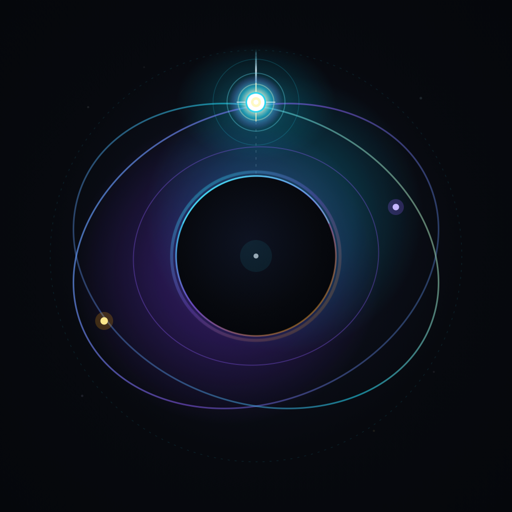
\includegraphics[width=1.35in]{app_icon.png}\\[1.2em]
  {\sffamily\huge\bfseries\color{CosmicDeep} AETHERIUM}\\[0.5em]
  {\large\itshape\color{AetherCyanDark} Where Celestial Physics Meets Receptive Music Therapy}\\[0.4em]
  {\sffamily\small\color{SlateMuted} The Official Companion eBook, Clinical Architecture Guide \& User Manual}\\[1.5em]
  {\sffamily\normalsize\bfseries By Drago\textcommabelow{s} Iorgulescu}\\
  {\sffamily\small Voidwave Lab $\cdot$ \href{https://github.com/voidwave-lab}{github.com/voidwave-lab}}
\end{center}

\vfill

\begin{tcolorbox}[colback=BoxBg, colframe=BoxBorder, arc=4pt, boxrule=0.5pt]
\footnotesize
\textbf{Copyright \copyright\ 2026 Drago\textcommabelow{s} Iorgulescu / Voidwave Lab.}\\[0.4em]
\textbf{Software \& Companion Book License:} \textit{Aetherium} is free software released under the \textbf{GNU General Public License v3.0 (or later)} (\texttt{GPL-3.0-or-later}), with an explicit GPLv3 Section 7 Additional Permission for mobile app store distribution (Apple App Store, TestFlight, Google Play, and F-Droid). You are free to run, study, share, and modify the software for personal, academic, or clinical use.\\[0.4em]
\textbf{Project Repository:} \url{https://github.com/voidwave-lab/Aetherium}\\
\textbf{Voidwave Lab Organization:} \url{https://github.com/voidwave-lab}\\
\textbf{Instant Mobile Web / PWA ("Aetherium Pocket"):} \url{https://voidwave-lab.github.io/Aetherium/pocket.html}\\[0.4em]
\textbf{Clinical \& Therapeutic Disclaimer:} \textit{Aetherium} and its \textit{Practitioner / Guide} suite are receptive music therapy and psychoacoustic co-regulation aids designed to support qualified mental health professionals, music therapists, and personal nervous-system self-regulation. It is \textbf{not} a medical device nor a substitute for professional medical diagnosis, psychotherapy, or psychiatric treatment.
\end{tcolorbox}

\clearpage

% --- Table of Contents ---
\tableofcontents
\clearpage

% ============================================================================
% MAIN MATTER (Arabic Page Numbering)
% ============================================================================
\mainmatter

% ============================================================================
% CHAPTER 1: GENESIS
% ============================================================================
\chapter[Genesis: From Hardware to Sanctuary]{Genesis: From Hardware Synthesizers to a Living Sanctuary}

\section{An Electronic Musician's Paradox}

\textbf{Aetherium} was not born in a corporate product roadmap or a venture-backed wellness startup. It emerged from a deeply personal necessity experienced by its creator, \textbf{Drago\textcommabelow{s} Iorgulescu}.

Having spent years immersed in electronic music equipment---working hands-on with hardware synthesizers, oscillators, resonant analog filters, step sequencers, modulation matrices, and effects processors---Drago\textcommabelow{s} knew firsthand the profound power of synthesized sound. When you dial in a slow-breathing low-pass filter over a detuned sawtooth drone, or route a delicate frequency-modulated (FM) pluck through a cavernous, pitch-drifting tape delay, the sound ceases to be mere entertainment. It becomes an acoustic architecture capable of slowing down racing thoughts, softening somatic tension in the chest, and anchoring a turbulent mind.

Yet living with acute anxiety states and unpredictable mood swings revealed a painful paradox at the heart of traditional electronic music instruments.

\begin{sanctuarybox}{The Friction Barrier in Moments of Dysregulation}
When your nervous system is locked in sympathetic hyperarousal---when anxiety spikes or a sudden mood swing leaves you exhausted, overwhelmed, or emotionally raw---your cognitive executive function drops sharply. In those exact moments when a warm, regulating soundscape is needed most, the last thing a human being can tolerate is technical friction:
\begin{itemize}
  \item Powering on a desk full of hardware synthesizers, routing MIDI and audio patch cables, and calibrating gain stages;
  \item Opening a complex Digital Audio Workstation (DAW), staring at a rigid horizontal timeline grid, browsing thousands of presets, or programming piano-roll sequences;
  \item Listening to static, pre-recorded streaming playlists whose predictable 3-minute loops quickly trigger auditory habituation and subconscious anticipation.
\end{itemize}
\end{sanctuarybox}

Drago\textcommabelow{s} realized that what he needed---and what millions of other people navigating anxiety, sensory overload, and emotional fluctuations needed---was a bridge between two worlds that rarely speak to each other: the deep, uncompromising acoustic craftsmanship of studio synthesis and the effortless, tactile immediacy of a contemplative sanctuary.

\section{Distilling Studio Craft into Celestial Motion}

The guiding question behind \textbf{Aetherium} became simple yet ambitious:
\begin{quote}
\itshape
``How can we translate decades of synthesizer design, physical modeling, and psychoacoustic research into an accessible, generative instrument where anyone---within three seconds of opening the app---can shape a living, never-repeating soundscape capable of regulating their emotional state?''
\end{quote}

To achieve this, Aetherium abandons the intimidating metaphors of traditional audio software. There are no tracks, no bars and beats, no mixer channels, and no technical jargon like \textit{cutoff}, \textit{resonance}, \textit{wet/dry mix}, or \textit{LFO rate}.

Instead, Aetherium reimagines the synthesizer as a \textbf{gravitational sky}:
\begin{enumerate}
  \item \textbf{The Breathing Core:} At the center of the canvas sits a warm celestial attractor whose harmonic pad and resonant filter expand and contract on a slow $0.05\text{--}0.15\text{ Hz}$ respiratory cycle ($6.6$ to $20$ seconds per breath), offering an immediate visual and acoustic pacing cue for slow diaphragmatic breathing.
  \item \textbf{Keplerian Harmonic Satellites:} Clicking anywhere in the dark space places an orbiting satellite. Governed by Kepler's laws of elliptical planetary motion, inner satellites orbit briskly and sing in delicate upper octaves, while outer satellites drift slowly and resonate in deep cello and bass registers.
  \item \textbf{The 12 O'Clock Meridian (\texttt{XII}):} Whenever a satellite crosses the glowing vertical meridian directly above the Core, it triggers a musical note mathematically quantized to a consonant harmonic scale. It is physically impossible to play a harsh or ``wrong'' note.
  \item \textbf{Six Poetic Macros:} Rather than exposing dozens of intimidating synthesizer knobs, the entire multi-layer DSP graph is sculpted through six intuitive poetic dimensions: \textbf{Luminance}, \textbf{Fog}, \textbf{Viscosity}, \textbf{Nostalgia}, \textbf{Rarity}, and \textbf{Serendipity}.
\end{enumerate}

\section{Why 100\% Procedural Audio Matters for the Nervous System}

Most relaxation apps rely on looping pre-recorded \texttt{.mp3} files of rain or ambient pads. To a hypervigilant or anxious brain, recorded loops present a subtle problem: within minutes, the auditory cortex detects repeating transient patterns and seam boundaries. Instead of relaxing, the brain begins tracking the loop.

Because Drago\textcommabelow{s} approached Aetherium from an electronic music engineering background, every single sound in Aetherium---from the felt-hammer piano transients and bowed glass strings to the Tibetan singing bowl partials, cathedral choir vowels, and distant rain on felt---is synthesized \textbf{100\% procedurally in real time} using mathematical oscillators, waveguide networks, and noise filters. No two minutes of Aetherium are ever identical.

% ============================================================================
% CHAPTER 2: ONE INSTRUMENT, TWO WORLDS
% ============================================================================
\chapter[One Sanctuary, Two Worlds]{One Sanctuary, Two Worlds: Everyday Listeners \& Clinical Practitioners}

As Aetherium evolved from a personal tool for anxiety and mood regulation, it became clear that the exact mechanisms that make generative music effective for personal self-regulation are rooted in decades of clinical research in \textbf{Receptive Music Therapy}, \textbf{Polyvagal Theory}, and \textbf{Eye Movement Desensitization and Reprocessing (EMDR)}.

Rather than forcing clinical tools onto casual listeners---or stripping away clinical precision for professionals---Aetherium greets you with a clean choice between two tailored spaces (switchable at any moment from the top bar):

\begin{center}
\begin{tabularx}{\textwidth}{>{\bfseries\sffamily\color{CosmicDeep}}p{1.65in} X}
\toprule
\textbf{Space Mode} & \textbf{Primary Audience \& Design Focus} \\
\midrule
Solo Explorer\newline{\footnotesize\normalfont\color{AetherCyanDark}(Personal Sanctuary)} &
Everyday individuals seeking immediate anxiety relief, mood stabilization, neurodivergent sensory grounding, deep focus, or restorative sleep---requiring zero musical or technical background. \\[0.6em]
Practitioner / Guide\newline{\footnotesize\normalfont\color{AetherEmeraldDark}(Clinical Suite)} &
Psychologists, psychiatrists, psychotherapists, EMDR practitioners, and music therapists conducting talk therapy, autonomic co-regulation, somatic grounding, and trauma processing with patients. \\
\bottomrule
\end{tabularx}
\end{center}

\section{Designing for the Everyday Person (\textit{Solo Explorer})}

When an individual is experiencing a mood swing, racing thoughts, or emotional overwhelm, cognitive load must be kept near zero. In \textbf{Solo Explorer} mode:
\begin{itemize}
  \item \textbf{Guaranteed Harmonic Safety:} Every note triggered by an orbiting satellite is dynamically quantized by the \texttt{HarmonicEngine} to match the active scale and chord voicing. Listeners can freely place, drag, or dissolve satellites without fear of creating jarring dissonance.
  \item \textbf{Mood-Matched Starting Seeds:} Eight curated procedural synthesis seeds (\textit{Rain on Felt}, \textit{Deep Drift}, \textit{Subterranean}, \textit{Solar Wind}, \textit{Midnight Vinyl}, \textit{Singing Bowls}, \textit{Cathedral Choir}, and \textit{Bowed Glass \& Strings}) let users immediately enter an acoustic environment that resonates with how they feel right now.
  \item \textbf{Pocket Sanctuary Everywhere:} Through \textbf{Aetherium Pocket} (available as a 100\% offline Progressive Web App for iOS and Android, as well as a native Android \texttt{.apk}), the exact same synthesis engine lives in the user's pocket---complete with Lock Screen controls, gyroscope tilt responsiveness, battery guard, and a gentle sleep timer.
\end{itemize}

\section{Designing for Psychology \& Psychiatry (\textit{Practitioner / Guide})}

In clinical psychotherapy and psychiatry, playing conventional background music during a session often fails for four well-documented neuroacoustic reasons. Aetherium's collapsible \textbf{Practitioner Suite} addresses each of these clinical challenges directly:

\subsection{Solving Speech Masking: Vocal-Range Acoustic Carving ($1100\text{ Hz}$)}
\textbf{The Clinical Problem:} Standard ambient music is rich in midrange harmonics between $400\text{ Hz}$ and $2.5\text{ kHz}$---the exact frequency band of human vocal fundamentals and vowel formants. When music occupies this band during talk therapy, both clinician and patient subconsciously strain to parse speech prosody, increasing cognitive fatigue.

\textbf{The Aetherium Solution:} Inspired by Dr.\ Stephen Porges' \textbf{Polyvagal Theory} (2011), which highlights how human vocal prosody cues the ventral vagal complex of safety, toggling \textbf{Dialogue ON} engages a smooth, two-octave-wide parametric EQ pocket centered at $1100\text{ Hz}$ ($Q = 0.7$, adjustable from $0\text{ dB}$ to $-12\text{ dB}$). Spoken conversation between therapist and patient becomes effortless and crystal clear, while the room remains enveloped in comforting sub-bass warmth ($40\text{--}150\text{ Hz}$) and airy upper shimmer ($>3.5\text{ kHz}$).

\subsection{Automating the ISO Principle Across a Clinical Hour}
\textbf{The Clinical Principle:} Formulated by psychiatrist Dr.\ Ira Altshuler (1948) and expanded by Grocke \& Wigram (2007), the \textbf{ISO Principle} states that playing cheerful, bright music to a deeply depressed or acutely agitated patient often causes emotional rejection. Instead, therapeutic music must first \textit{mirror} the patient's current affective and autonomic state, and then gradually guide (\textit{vector}) them toward regulation.

\textbf{The Aetherium Solution:} Practitioners simply select their session duration ($20\text{m}$, $45\text{m}$, $50\text{m}$ clinical hour, or $60\text{m}$), choose \textbf{Phase 1 --- Mirroring} (\textit{High Agitation / Tension}, \textit{Melancholic / Heavy}, or \textit{Dissociated / Flat}), and choose \textbf{Phase 2 --- Co-Regulation} (\textit{Parasympathetic Rest} or \textit{Warm Openness}). Clicking \textbf{Start Session Arc} hands the controls to Aetherium's piecewise cosine vector engine, which smoothly morphs scale luminance, orbital speed, reverb mist, and serendipity across the entire session---including an automatic \textbf{Phase 3 --- Re-Orientation} during the final $10\%$ of the hour so the patient leaves the office alert and grounded.

\subsection{Synchronized Bilateral Grounding (EMDR) with Safety Locks}
\textbf{The Clinical Need:} During Eye Movement Desensitization and Reprocessing (EMDR; Shapiro, 2018) and somatic stabilization, clinicians use rhythmic left-right bilateral stimulation ($0.2\text{--}1.5\text{ Hz}$) to tax working memory and facilitate adaptive information processing.

\textbf{The Aetherium Solution:} Toggling \textbf{Bilateral Grounding} pans the harmonic voices and a soft root-tuned pulse smoothly between left and right audio channels while synchronizing cyan luminescence pillars and a horizontal tracking beacon on the canvas. Crucially, Aetherium includes a \textbf{Clinical Safety Guard}: the moment Bilateral EMDR mode is enabled, the \textbf{Serendipity} engine is automatically clamped to $0\%$ so random melodic sparks or shooting stars never distract the patient's ocular or auditory tracking.

\subsection{Somatic Sub-Bass ($40\text{--}60\text{ Hz}$), Binaural Theta ($6\text{ Hz}$) \& Take-Home Prescriptions}
For patients experiencing severe dissociation or somatic anxiety, practitioners can engage a pure \textbf{Somatic Sub-Bass Anchor} ($43.65\text{--}55\text{ Hz}$) that bypasses the speech-carving filter to provide gentle physical vibration in the room, or enable \textbf{$6\text{ Hz}$ Binaural Theta Entrainment} ($100\text{ Hz}$ Left / $106\text{ Hz}$ Right; Oster, 1973) for headphone sessions. Finally, using \textbf{Patient Take-Home Anchor}, clinicians can record a $3$-, $5$-, or $10$-minute seamless audio loop of the exact regulated state co-created in session and hand it to the patient as a \texttt{.wav} or mobile-ready \texttt{.webm} ``acoustic prescription'' for homework between appointments.

% ============================================================================
% CHAPTER 3: GENERATIVE MUSIC MECHANISMS & RESEARCH
% ============================================================================
\chapter[Generative Mechanisms \& DSP]{Generative Music Mechanisms \& Psychoacoustic Architecture}

Underneath its calm, minimalist surface, Aetherium is a deterministic real-time physics and digital signal processing (DSP) engine built with TypeScript, Web Audio API, Tone.js, Tonal, and a native Rust/Tauri core. This chapter explores how each generative mechanism works.

\section{System Architecture \& Signal Flow}

Aetherium is structured around four decoupled subsystems that communicate at $60\text{ frames per second}$ visually and sample-accurately in the audio thread:

\begin{center}
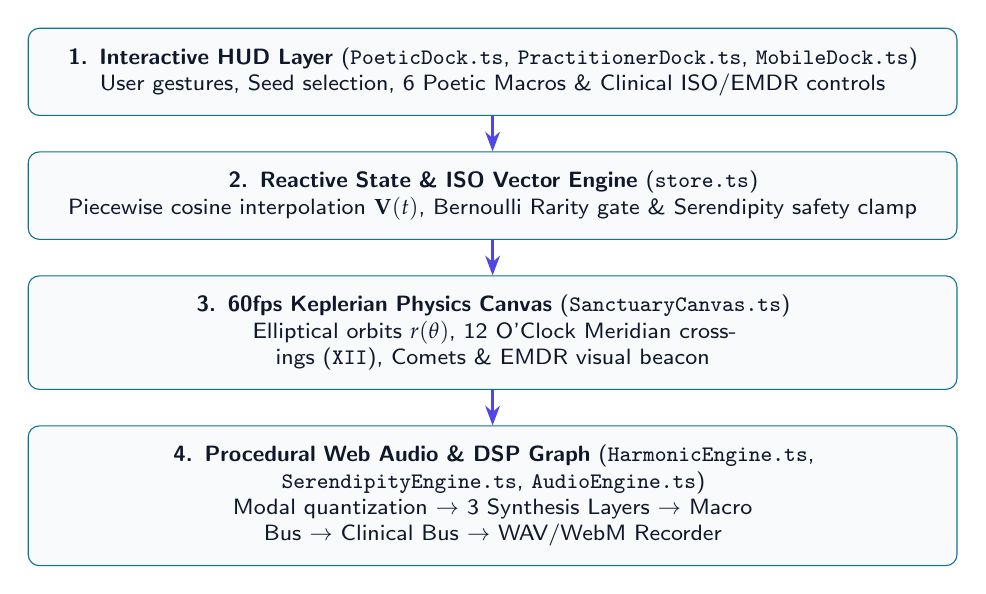
\begin{tikzpicture}[
  node distance=0.45cm and 0.6cm,
  box/.style={
    rectangle,
    rounded corners=4pt,
    draw=AetherCyanDark,
    fill=BoxBg,
    text=CosmicDeep,
    font=\sffamily\footnotesize,
    align=center,
    text width=4.45in,
    minimum width=4.6in,
    inner sep=7pt
  },
  arrow/.style={-{Stealth[length=2.5mm]}, thick, color=AetherIndigo}
]
  \node[box] (ui) {\textbf{1. Interactive HUD Layer} (\texttt{PoeticDock.ts}, \texttt{PractitionerDock.ts}, \texttt{MobileDock.ts})\\User gestures, Seed selection, 6 Poetic Macros \& Clinical ISO/EMDR controls};
  \node[box, below=of ui] (state) {\textbf{2. Reactive State \& ISO Vector Engine} (\texttt{store.ts})\\Piecewise cosine interpolation $\mathbf{V}(t)$, Bernoulli Rarity gate \& Serendipity safety clamp};
  \node[box, below=of state] (canvas) {\textbf{3. 60fps Keplerian Physics Canvas} (\texttt{SanctuaryCanvas.ts})\\Elliptical orbits $r(\theta)$, 12 O'Clock Meridian crossings (\texttt{XII}), Comets \& EMDR visual beacon};
  \node[box, below=of canvas] (audio) {\textbf{4. Procedural Web Audio \& DSP Graph} (\texttt{HarmonicEngine.ts}, \texttt{SerendipityEngine.ts}, \texttt{AudioEngine.ts})\\Modal quantization $\rightarrow$ 3 Synthesis Layers $\rightarrow$ Macro Bus $\rightarrow$ Clinical Bus $\rightarrow$ WAV/WebM Recorder};

  \draw[arrow] (ui) -- (state);
  \draw[arrow] (state) -- (canvas);
  \draw[arrow] (canvas) -- (audio);
\end{tikzpicture}
\end{center}

\section{Keplerian Orbital Physics \& The 12 O'Clock Meridian}

Rather than triggering notes along a rigid $4/4$ metronome grid---which can feel mechanical and pressuring to an anxious listener---Aetherium uses orbital mechanics (\texttt{SanctuaryCanvas.ts}).

Each of the up to $12$ user-placed satellites $i \in [1, 12]$ moves along an elliptical orbit defined by its normalized semi-major axis $a \in [0.14, 0.94]$, orbital eccentricity $e \in [0.04, 0.24]$, argument of periapsis $\omega$, and true anomaly angle $\theta \in [-\pi, \pi]$. Its instantaneous distance from the Central Core is governed by the Keplerian conic equation:
\[
  r(\theta) = \frac{a(1 - e^2)}{1 + e \cos(\theta - \omega)}
\]

Following Kepler's laws of planetary motion, a satellite's angular velocity is inversely proportional to its radial distance (tuned with an exponent of $1.42$ for expressive musical pacing) and modulated by both the \textbf{Viscosity} slider ($v \in [0, 1]$) and the \textbf{ISO-Principle Pace Multiplier} ($m_{\text{iso}}$):
\[
  \frac{d\theta}{dt} = \frac{k_0}{\max(0.14, r(\theta))^{1.42}} \cdot (1 - 0.68v) \cdot m_{\text{iso}}, \quad k_0 = 0.22\text{ rad/s}
\]

Directly above the Core at $\theta_{\text{meridian}} = -\frac{\pi}{2}$ (12 o'clock North) lies the glowing \textbf{Meridian (\texttt{XII})}. Whenever a satellite's trajectory crosses this line ($\theta_{t-1} < -\frac{\pi}{2} \le \theta_t$), the canvas fires an acoustic trigger event and spawns a concentric luminescence ripple. Because each satellite orbits at its own irrational period determined by its exact radial placement, the resulting polyrhythms evolve continuously without ever repeating a rigid bar structure.

\section{Harmonic Quantization \& Luminance Modal Morphing}

Implemented in \texttt{HarmonicEngine.ts} using the functional music-theory library \texttt{Tonal}, the \textbf{Luminance} slider ($L \in [0.0, 1.0]$) acts as an emotional brightness vector. Moving Luminance from \textit{Shadow} ($0.0$) to \textit{Light} ($1.0$) smoothly transitions both the active musical scale and the continuous 4-note Core Drone voicing through four psychoacoustic zones:

\begin{center}
\footnotesize
\begin{tabularx}{\textwidth}{l l l X}
\toprule
\textbf{Luminance} & \textbf{Zone ID} & \textbf{Musical Mode} & \textbf{Psychoacoustic \& Emotional Character} \\
\midrule
\texttt{0.00 -- 0.25} & \texttt{shadow-aeolian} & Aeolian / Phrygian & Grounded minor introspection; safe space for grief or heavy moods. \\
\texttt{0.25 -- 0.50} & \texttt{wistful-dorian} & Dorian ($\text{min7}/\text{add9}$) & Intimate, bittersweet warmth via the raised natural 6th and 9th. \\
\texttt{0.50 -- 0.75} & \texttt{floating-maj9} & Major Pentatonic / $\text{Maj9}$ & Open, reassuring consonance free of half-step tension. \\
\texttt{0.75 -- 1.00} & \texttt{cosmic-lydian} & Lydian ($\sharp 4 / \sharp 11$) & Expansive, weightless wonder driven by the raised fourth degree. \\
\bottomrule
\end{tabularx}
\end{center}

Furthermore, a satellite's orbital radius $a$ automatically determines its pitch octave:
\begin{itemize}
  \item \textbf{Inner Orbits ($0.14 \le a < 0.38$):} Crystalline upper register (\textbf{Octaves 4--5}).
  \item \textbf{Middle Orbits ($0.38 \le a < 0.68$):} Warm midrange body (\textbf{Octaves 3--4}).
  \item \textbf{Outer Orbits ($0.68 \le a \le 0.94$):} Deep cello and bass register (\textbf{Octaves 2--3}).
\end{itemize}

Before any Meridian crossing produces sound, Aetherium evaluates a Bernoulli trial against the \textbf{Rarity} slider ($R \in [0, 1]$), where $P(\text{silence}) = 0.90 \cdot R$. When silenced by Rarity, the satellite renders a quiet \texttt{silence} ripple without playing a note---honoring Brian Eno's and Miles Davis's insight that silence is as vital to calm as sound.

\section{The Eight Procedural Seeds \& Six Synthesis Engines}

Every sound in Aetherium is generated by three simultaneous synthesis layers in \texttt{AudioEngine.ts}:
\begin{enumerate}
  \item \textbf{Layer A (The Respiratory Core Drone):} A 3-oscillator detuned \texttt{fatsawtooth} pad ($24\text{ cents}$ spread) paired with a $-12\text{ dB}$ sub-fundamental sine wave, routed through a resonant $24\text{ dB/oct}$ low-pass filter swept by a $0.05\text{--}0.15\text{ Hz}$ breathing LFO.
  \item \textbf{Layer B (Six Specialized Polyphonic Synthesis Architectures):}
    \begin{itemize}
      \item \textbf{FM Felt Piano (\textit{Rain on Felt}, \textit{Subterranean}):} 2-operator FM synthesis (\texttt{harmonicity: 2.0}) with soft felt-hammer attack transients and warm woody decay.
      \item \textbf{AM Glassy Space Pad (\textit{Deep Drift}, \textit{Solar Wind}):} Dual \texttt{fatsine} carriers with fifth-overtone AM shimmer (\texttt{harmonicity: 1.5}) and slow $1.5\text{--}4.0\text{s}$ swells.
      \item \textbf{Nocturnal Lo-Fi / Future Garage (\textit{Midnight Vinyl}):} Warm Rhodes FM dyads filtered below $600\text{ Hz}$, paired with a $55\text{ Hz}$ sub-bass anchor and stochastic $2.5\text{ kHz}$ vinyl micro-impulses.
      \item \textbf{Inharmonic Modal Resonance (\textit{Singing Bowls}):} Four parallel sine banks tuned to Euler-Bernoulli metallic bar/bowl mode ratios ($[1.000, 2.756, 5.404, 8.933] \times f_0$; Smith, 2010) with a $0.08\text{s}$ felt-mallet strike and $14\text{s}$ shimmer decay.
      \item \textbf{Vowel Formant Synthesis (\textit{Cathedral Choir}):} A 4-voice detuned sawtooth choir routed through three parallel high-$Q$ formant bandpass filters ($F_1, F_2, F_3$) that morph continuously between sung vowel \texttt{`Ahh'} ($[700, 1220, 2600\text{ Hz}]$) and \texttt{`Ooo'} ($[450, 800, 2830\text{ Hz}]$).
      \item \textbf{Karplus-Strong \& Bowed Strings (\textit{Bowed Glass \& Strings}):} Combines a $3.0\text{s}$ slow-attack bowed synth with a physical-modeling Karplus-Strong plucked string (\texttt{Tone.PluckSynth}; Karplus \& Strong, 1983) routed through a 3-band woody cello body filter bank ($250\text{ Hz}$, $520\text{ Hz}$, $1850\text{ Hz}$) with $4.5\text{ Hz}$ vibrato.
    \end{itemize}
  \item \textbf{Layer C (Procedural Organic Texture):} Dual pink and brown noise generators swept by a $0.065\text{ Hz}$ bandpass filter ($240\text{--}1180\text{ Hz}$; Farnell, 2010), creating non-looping rain on felt, wind through pines, and warm room air.
\end{enumerate}

\section{Poetic Macro DSP \& The Serendipity Engine}

All synthesis layers flow through the \textbf{Poetic Macro DSP Bus}:
\begin{itemize}
  \item \textbf{Fog ($F \in [0, 1]$):} Expands a cascaded Freeverb + Convolution Reverb network from $2\text{s}$ to an $18\text{s}$ cathedral tail while exponentially rolling off the master low-pass filter from $12\text{ kHz}$ down to $1.2\text{ kHz}$:
  {\small\[
    f_{\text{fog}}(F, L) = \operatorname{clamp}\!\left(12000 \cdot \left(\frac{1200}{12000}\right)^F \cdot (0.75 + 0.50L),\ 950,\ 14000\right)\text{ Hz}
  \]}
  \item \textbf{Nostalgia ($N \in [0, 1]$):} Inspired by William Basinski's \textit{The Disintegration Loops} (2002), modulates a $12\text{ ms}$ delay line by $\pm 3.8N\text{ ms}$ at $0.8\text{ Hz}$ for authentic analog tape \textit{wow \& flutter}, followed by a hyperbolic tangent waveshaper $y(x) = \tanh(kx)/\tanh(k)$ ($k = 0.6 + 2.2N$) for warm harmonic saturation.
\end{itemize}

Finally, to prevent auditory habituation over long listening sessions without ever startling a resting user, \texttt{SerendipityEngine.ts} schedules gentle stochastic events at intervals $[T_{\min}, T_{\max}]$ inversely scaled by the \textbf{Serendipity} slider ($S \in [0, 1]$):
\begin{enumerate}
  \item \textbf{Rubato Arpeggio (60\% probability):} Plays $3$ to $5$ consonant scale extensions (Root, 5th, 7th, 9th, 11th) with a human-like decelerating tempo ($\Delta t_i \in [350, 900]\text{ ms}$), synchronized with a \textbf{Shooting Star Comet} gliding across the outer sky.
  \item \textbf{Modal Breeze (20\% probability):} Gently shifts the harmonic root to the Subdominant ($\text{IV}$) or Submediant ($\text{VI}$) degree for $16\text{--}24\text{ seconds}$ before returning home to $\text{I}$, accompanied by an expanding \textbf{Aurora Ripple} from the Core.
  \item \textbf{High-Octave Shimmer (20\% probability):} Breathes a 100\%-wet reverberant 5th or 3rd dyad in Octave 5 alongside a translucent halo in the upper canopy.
\end{enumerate}

% ============================================================================
% CHAPTER 4: GETTING STARTED
% ============================================================================
\chapter[Getting Started]{Getting Started: Installation \& First Launch}

You do not need any programming knowledge or external audio equipment to install and enjoy Aetherium. It runs 100\% offline on desktop computers, phones, and tablets.

\section{Downloading \& Installing on Your Device}

All official, cryptographically signed releases are provided free of charge on the Voidwave Lab GitHub Releases page:
\begin{center}
  \url{https://github.com/voidwave-lab/Aetherium/releases}
\end{center}

\subsection{Desktop Installation (macOS, Windows \& Linux)}
\begin{itemize}
  \item \textbf{macOS (Apple Silicon M1 / M2 / M3 / M4):}\\
  Download \texttt{Aetherium\_0.4.0\_aarch64.dmg}.
  \item \textbf{macOS (Intel Mac):}\\
  Download \texttt{Aetherium\_0.4.0\_x64.dmg}.
    \begin{itemize}
      \item \textit{macOS First-Launch Tip:} Open the \texttt{.dmg} file and drag \textbf{Aetherium} into your \textbf{Applications} folder. If macOS Gatekeeper shows an \textit{``unidentified developer''} dialog on first launch, simply \textbf{Right-Click (or Control-Click) \texttt{Aetherium.app} $\rightarrow$ select Open}.
    \end{itemize}
  \item \textbf{Windows (Windows 10 / 11):}\\
  Download \texttt{Aetherium\_0.4.0\_x64-setup.exe} (or the \texttt{.msi} installer) and double-click to install. If Windows SmartScreen appears, click \textbf{More info $\rightarrow$ Run anyway}.
  \item \textbf{Linux (Ubuntu, Debian, Mint, Fedora):}\\
  Download \texttt{Aetherium\_0.4.0\_amd64.AppImage}, mark it executable (\texttt{chmod +x Aetherium*.AppImage}), and run it directly---or install the Debian package:\\
  \texttt{sudo dpkg -i Aetherium\_0.4.0\_amd64.deb}.
\end{itemize}

\subsection{Mobile Installation ("Aetherium Pocket" for iOS \& Android)}
\begin{itemize}
  \item \textbf{Instant Offline PWA (iOS Safari \& Android Chrome):} Visit \url{https://voidwave-lab.github.io/Aetherium/pocket.html} on your phone or tablet. Tap \textbf{Share $\rightarrow$ Add to Home Screen} (iOS) or \textbf{Install App} (Android). Aetherium Pocket installs as a full-screen portrait app that works 100\% offline on airplanes or in clinics, complete with Lock Screen playback controls, Battery Guard, Gyroscope Tilt modulation, and an overnight Sleep Timer.
  \item \textbf{Native Android APK:} Download \texttt{Aetherium-Pocket.apk} directly from the GitHub Releases page to install the standalone Capacitor Android build.
\end{itemize}

\section{First Launch: Navigating the Sanctuary Interface}

When you open Aetherium for the first time, the \textbf{Select Your Space} glass modal invites you to choose between \textbf{Solo Explorer} and \textbf{Practitioner / Guide}. Don't worry about making a permanent choice---you can switch between the two modes at any time using the mode switcher pill in the top-right corner of the window.

The interface is organized into four serene zones:
\begin{enumerate}
  \item \textbf{Top Telemetry \& Preset Bar:} Displays your current musical scale and root note, active satellite count, the \textbf{Save / Load (\texttt{.aether.json})} preset buttons, the \textbf{Ethics, Credits \& Bibliography (\texttt{i})} button, and the \textbf{Solo Explorer $\leftrightarrow$ Practitioner / Guide} mode switcher.
  \item \textbf{The Central Orbital Canvas:} Your interactive sky containing the breathing Central Core, the 12 O'Clock Meridian (\texttt{XII}), and up to 12 orbiting harmonic satellites.
  \item \textbf{The Bottom Poetic Dock:} Houses the \textbf{Awaken Audio / Mute} button, \textbf{Capture Sanctuary} live audio recorder, \textbf{Fade to Silence} sleep timer ($15\text{m}$ / $30\text{m}$ / $60\text{m}$), the \textbf{8 Procedural Seeds}, and the \textbf{6 Poetic Macro Sliders}.
  \item \textbf{The Collapsible Practitioner Dock (Right Panel):} Visible when \textbf{Practitioner / Guide} mode is active, providing instant access to Vocal-Range Carving, the ISO-Principle Session Arc, Bilateral EMDR Grounding, Somatic Sub-Bass, Binaural Theta, and the Patient Take-Home Anchor recorder.
\end{enumerate}

% ============================================================================
% CHAPTER 5: TUTORIALS
% ============================================================================
\chapter[Hands-On Tutorials]{Hands-On Tutorials: Self-Regulation \& Clinical Workflows}

This chapter provides four step-by-step tutorials designed to help you get the most out of Aetherium---whether you are regulating your own anxiety at midnight or guiding a patient through a 50-minute psychotherapy session.

\section{Tutorial 1 (Solo Explorer): Rapid Anxiety Relief \& Mood Grounding in 60 Seconds}

\textbf{Goal:} Quickly calm a racing mind or sudden anxiety spike without musical effort.

\begin{enumerate}
  \item \textbf{Enter Solo Explorer \& Awaken the Sanctuary:} Launch Aetherium, choose \textbf{Solo Explorer}, and put on comfortable headphones or turn on warm room speakers. Click \textbf{Awaken Audio} in the bottom-left dock.
  \item \textbf{Sync Your Breath with the Core:} Before placing a single note, watch the glowing \textbf{Central Core} at the center of the screen. Notice how it gently expands and contracts every 10 to 15 seconds in exact synchrony with the warm low-pass filter swell. Take three slow breaths following the Core's expansion and contraction.
  \item \textbf{Choose a Grounding Seed:} In the bottom dock, select \textbf{Rain on Felt} (for intimate, comforting warmth) or \textbf{Singing Bowls} (for deep somatic resonance).
  \item \textbf{Place 3 to 4 Orbiting Satellites:}
    \begin{itemize}
      \item Click once \textbf{far from the Core} (outer ring) to spawn a slow-moving bass/cello satellite that anchors the room in Octave 2--3.
      \item Click twice in the \textbf{middle zone} to add warm midrange harmony notes in Octave 3--4.
      \item Click once \textbf{close to the Core} to add a gentle upper-octave melody note.
    \end{itemize}
    Watch as each satellite glides clockwise and triggers a consonant note every time it crosses the vertical \textbf{12 O'Clock Meridian (\texttt{XII})}.
  \item \textbf{Soften the Sky with Poetic Macros:}
    \begin{itemize}
      \item Set \textbf{Luminance} to around \texttt{35\%--45\%} (\textit{Wistful Dorian}) if you feel heavy or anxious and want a gentle, validating embrace, or \texttt{65\%} (\textit{Floating Maj9}) for reassuring warmth.
      \item Raise \textbf{Fog} to \texttt{70\%} to wrap the notes in a deep, mist-like cathedral reverb and soften sharp high frequencies.
      \item Raise \textbf{Viscosity} to \texttt{65\%} to slow down the orbital pace and turn note attacks into gentle swells.
      \item Raise \textbf{Rarity} to \texttt{30\%} so satellites occasionally rest in silence when crossing the Meridian, giving your mind space to breathe.
    \end{itemize}
\end{enumerate}

\section{Tutorial 2 (Solo Explorer): Nocturnal Drift \& Recording a Seamless Loop}

\textbf{Goal:} Create an evolving nocturnal soundscape and record a studio-quality loop for offline listening on your phone.

\begin{enumerate}
  \item \textbf{Select a Nocturnal Seed:} Click \textbf{Midnight Vinyl} (for warm $<600\text{ Hz}$ Rhodes chords, $55\text{ Hz}$ sub-bass, and subtle vinyl crackle) or \textbf{Bowed Glass \& Strings} (for cinematic slow-bowed harmonies).
  \item \textbf{Dial in Analog Warmth \& Living Sparks:}
    \begin{itemize}
      \item Increase \textbf{Nostalgia} to \texttt{55\%} to introduce subtle analog tape \textit{wow \& flutter} pitch drift and warm harmonic saturation.
      \item Set \textbf{Serendipity} to \texttt{45\%}. Every 12 to 18 seconds, Aetherium will surprise you with a soft \textit{Rubato Arpeggio} accompanied by a shooting star across the outer canvas, or a 20-second \textit{Modal Breeze} harmonic shift to $\text{IV}$ or $\text{VI}$ with an aurora ripple.
    \end{itemize}
  \item \textbf{Reshape Your Constellation:} Drag any inner satellite slightly outward if it feels too busy, or \textbf{right-click} (press-and-hold on mobile) a satellite to dissolve it into stardust. Drag the \textbf{Central Core} slightly left or right to shift the stereo center.
  \item \textbf{Record Your Sanctuary:}
    \begin{itemize}
      \item Click \textbf{Capture Sanctuary} in the bottom dock. An amber/crimson breathing indicator and \texttt{MM:SS} timer will appear.
      \item Let your soundscape play for 3 to 5 minutes, then click \textbf{Stop Capture}.
      \item In the export modal, choose \textbf{Lossless Studio (\texttt{.wav})} or \textbf{Mobile Compact (\texttt{.webm})}. Aetherium automatically applies a \textbf{2-second cosine fade-in} and \textbf{3-second cosine fade-out} so you can put the exported file on repeat on your phone with zero clicks or pops!
    \end{itemize}
\end{enumerate}

\section{Tutorial 3 (Practitioner / Guide): Conducting a 50-Minute Talk Therapy Session with the ISO Principle}

\textbf{Goal:} Provide an emotionally regulating acoustic environment during spoken psychotherapy or psychiatric consultation without interfering with speech intelligibility.

\begin{clinicalbox}{Clinical Setup Checklist for Talk Therapy}
\begin{enumerate}
  \item \textbf{Switch to Practitioner / Guide Mode:} Click the mode pill in the top-right corner so the \textbf{Practitioner Suite} opens on the right side of the screen.
  \item \textbf{Engage Vocal-Range Carving (Section 1):} Toggle \textbf{Dialogue ON} and set the carving depth to \texttt{-8 dB} (or \texttt{-10 dB} for quieter speakers). Notice how the midrange ($400\text{ Hz} \text{--} 2.5\text{ kHz}$) immediately opens up, leaving spoken voices between you and your patient completely clear and effortless.
  \item \textbf{Configure the Automated ISO-Principle Session Arc (Section 2):}
    \begin{itemize}
      \item Select \textbf{\texttt{50m}} (standard clinical hour).
      \item Under \textbf{Phase 1 --- Mirroring (Start State)}, select the profile that matches how your patient arrives in the room (e.g., \textit{High Agitation / Tension} if they arrive anxious and rapid, or \textit{Melancholic / Heavy} if they arrive with depressed affect).
      \item Under \textbf{Phase 2 --- Co-Regulation (75\% Target State)}, select \textit{Parasympathetic Rest / Safe Grounding}.
      \item Click \textbf{Start Session Arc}.
    \end{itemize}
  \item \textbf{Focus 100\% on Your Patient:} Over the next 50 minutes, you do not need to touch the computer once:
    \begin{itemize}
      \item \textbf{Minutes 0--37 (Mirroring $\rightarrow$ Co-Regulation):} Aetherium begins in a state that validates the patient's initial affect and smoothly cosine-interpolates orbital velocity, modal scale, and reverb mist toward deep parasympathetic rest.
      \item \textbf{Minutes 37--45 (Consolidation Plateau):} Holds the calm, grounded target state steady while keeping \textbf{Serendipity} low (\texttt{5\%}).
      \item \textbf{Minutes 45--50 (Phase 3 --- Re-Orientation):} Automatically brightens \textbf{Luminance} toward \texttt{84\%}, clears the \textbf{Fog} to \texttt{22\%}, and gently raises \textbf{Serendipity} to \texttt{35\%} so the patient is softly re-oriented and alert before stepping out of your office.
    \end{itemize}
\end{enumerate}
\end{clinicalbox}

\section{Tutorial 4 (Practitioner / Guide): Bilateral EMDR Grounding \& Prescribing a Take-Home Anchor}

\textbf{Goal:} Use synchronized auditory/visual bilateral stimulation for somatic grounding or EMDR, and give the patient a 5-minute take-home audio prescription.

\begin{enumerate}
  \item \textbf{Activate Bilateral Grounding (Section 3):} In the Practitioner Suite, toggle \textbf{Bilateral Grounding} to \textbf{ON}.
  \item \textbf{Calibrate Rate \& Stereo Width:}
    \begin{itemize}
      \item For slow somatic resourcing and grounding, set \textbf{Sweep Rate} between \texttt{0.2 Hz} and \texttt{0.5 Hz}.
      \item For active bilateral processing, adjust between \texttt{0.8 Hz} and \texttt{1.5 Hz}, with \textbf{Stereo Width} at \texttt{80\%--100\%}.
      \item Notice that the \textbf{Serendipity Auto-Lock} badge illuminates automatically, clamping random musical/visual sparks to \texttt{0\%} so the patient's bilateral tracking is never interrupted.
    \end{itemize}
  \item \textbf{Optional Somatic Sub-Bass (Section 4):} If the patient feels ungrounded or dissociated, raise the \textbf{Somatic Sub-Bass ($40\text{--}60\text{ Hz}$)} slider to \texttt{45\%} to add a comforting physical sub-fundamental anchor.
  \item \textbf{Export a Patient Take-Home Anchor (Section 5):} At the end of the session, scroll to \textbf{5.\ Patient Take-Home Anchor} and click \textbf{\texttt{Capture 5 Min Anchor}}. When the progress bar finishes (or when you click \textbf{Finish \& Export Now}), choose \textbf{Mobile Compact (\texttt{.webm})} to send directly to the patient via email or messaging, or \textbf{Lossless Studio (\texttt{.wav})}.
\end{enumerate}

% ============================================================================
% CHAPTER 6: RESEARCH BIBLIOGRAPHY
% ============================================================================
\chapter[Research \& Bibliography]{Foundational Research \& Academic Bibliography}

Aetherium stands on the shoulders of more than seven decades of peer-reviewed research in digital signal processing, physical modeling acoustics, generative music composition, psychiatry, and receptive music therapy. Below is the complete annotated bibliography of the works that directly shaped Aetherium's algorithms.

\section{Digital Signal Processing \& Physical Modeling Synthesis}

\begin{enumerate}[label=\textbf{[\arabic*]}]
  \item \textbf{Karplus, K., \& Strong, A. (1983).} ``Digital Synthesis of Plucked-String and Drum Timbres.'' \textit{Computer Music Journal}, 7(2), 43--55.\\
  \textit{Implementation in Aetherium:} Forms the mathematical foundation for the sympathetic plucked string and harp resonance in the \textbf{Bowed Glass \& Strings} synthesis engine (\texttt{AudioEngine.ts}), using short delay-line waveguides excited by filtered noise bursts.

  \item \textbf{Smith, J.\ O. (2010).} \textit{Physical Audio Signal Processing: For Virtual Musical Instruments and Audio Effects.} W3K Publishing / Center for Computer Research in Music and Acoustics (CCRMA), Stanford University.\\
  \textit{Implementation in Aetherium:} Provides the Euler-Bernoulli metallic beam/bowl modal frequency ratios ($[1.000, 2.756, 5.404, 8.933] \times f_0$) used in the \textbf{Singing Bowls} engine, the parallel vocal-tract formant resonators ($F_1, F_2, F_3$) morphing between \texttt{`Ahh'} and \texttt{`Ooo'} in \textbf{Cathedral Choir}, and the 3-band woody cello body filter bank.

  \item \textbf{Farnell, A. (2010).} \textit{Designing Sound.} MIT Press.\\
  \textit{Implementation in Aetherium:} Guides Aetherium's zero-sample procedural soundscaping philosophy---synthesizing continuous rain on felt, wind through pines, and stochastic $2.5\text{ kHz}$ vinyl micro-impulses purely from mathematically filtered pink and brown noise sources.

  \item \textbf{Roads, C. (2001).} \textit{Microsound.} MIT Press.\\
  \textit{Implementation in Aetherium:} Informs the stochastic event scheduling, Poisson/uniform cloud spacing, and high-octave shimmer grain envelopes in \texttt{SerendipityEngine.ts}.
\end{enumerate}

\section{Generative \& Ambient Music Theory}

\begin{enumerate}[label=\textbf{[\arabic*]}, resume]
  \item \textbf{Eno, B. (1978).} \textit{Ambient 1: Music for Airports} (Liner Notes \& Generative Music Manifesto). Editions EG.\\
  \textit{Implementation in Aetherium:} Establishes the core philosophical definition of ambient music as an acoustic environment \textit{``able to accommodate many levels of listening attention without enforcing one in particular; as ignorable as it is interesting''}---realized in Aetherium through asynchronous Keplerian orbital periods that never repeat a static loop.

  \item \textbf{Basinski, W. (2002).} \textit{The Disintegration Loops.} 2062 Records.\\
  \textit{Implementation in Aetherium:} Inspires the \textbf{Nostalgia} macro ($0.8\text{ Hz}$ tape \textit{wow \& flutter} delay modulation, $\tanh$ soft-clipping warmth, and procedural sepia film grain) as well as the \textbf{Rarity} probabilistic entropy gate ($P(\text{silence}) = 0.90 R$), where notes gracefully dissolve into silence.
\end{enumerate}

\section{Receptive Music Therapy, Polyvagal Theory \& Clinical Psychoacoustics}

\begin{enumerate}[label=\textbf{[\arabic*]}, resume]
  \item \textbf{Altshuler, I.\ M. (1948).} ``A Psychiatrist's Experience with Music as a Therapeutic Agent.'' In D.\ M.\ Schullian \& M.\ Schoen (Eds.), \textit{Music and Medicine} (pp.\ 266--281). Henry Schuman.\\
  \textit{Implementation in Aetherium:} Introduces the clinical \textbf{ISO Principle} in psychiatry---demonstrating that therapeutic sound must first match (\textit{mirror}) a patient's internal affective and autonomic state before gradually vectoring them toward regulation. Directly implemented in Aetherium's 6-dimensional piecewise cosine interpolation engine (\texttt{evaluateIsoSessionArc} in \texttt{store.ts}).

  \item \textbf{Grocke, D., \& Wigram, T. (2007).} \textit{Receptive Methods in Music Therapy: Techniques and Clinical Applications for Music Therapy Clinicians, Educators and Students.} Jessica Kingsley Publishers.\\
  \textit{Implementation in Aetherium:} Defines clinical protocols for receptive soundscaping, parasympathetic consolidation plateaus, and structured \textbf{Phase 3 Re-Orientation} during the final $10\%$ of a clinical session.

  \item \textbf{Porges, S.\ W. (2011).} \textit{The Polyvagal Theory: Neurophysiological Foundations of Emotions, Attachment, Communication, and Self-Regulation.} W.\ W.\ Norton \& Company.\\
  \textit{Implementation in Aetherium:} Provides the neurophysiological basis for Aetherium's \textbf{Vocal-Range Acoustic Carving ($1100\text{ Hz}$, $Q=0.7$)} in Dialogue Mode---preventing background music from masking the human prosodic vocal frequency band ($400\text{ Hz} \text{--} 2.5\text{ kHz}$) that signals social safety to the ventral vagal complex, as well as the $0.05\text{--}0.15\text{ Hz}$ respiratory Core filter pacing.

  \item \textbf{Shapiro, F. (2018).} \textit{Eye Movement Desensitization and Reprocessing (EMDR) Therapy: Basic Principles, Protocols, and Procedures} (3rd ed.). Guilford Press.\\
  \textit{Implementation in Aetherium:} Forms the clinical basis for Aetherium's synchronized $0.2\text{--}1.5\text{ Hz}$ \textbf{Bilateral Auditory \& Visual Stimulation} panner and the automatic \textbf{Serendipity Distraction Guard} that clamps random melodic/visual events to $0\%$ while bilateral processing is active.

  \item \textbf{Oster, G. (1973).} ``Auditory Beats in the Brain.'' \textit{Scientific American}, 229(4), 94--102.\\
  \textit{Implementation in Aetherium:} Establishes the neuroacoustic mechanism for dichotic low-frequency binaural beat perception in the superior olivary complex, implemented in Aetherium's \textbf{Binaural Theta ($6\text{ Hz}$)} headphone entrainment module ($100\text{ Hz}$ Left / $106\text{ Hz}$ Right).
\end{enumerate}

% ============================================================================
% CHAPTER 7: VOIDWAVE LAB, ETHICS & LICENSING
% ============================================================================
\chapter[Voidwave Lab \& Licensing]{Voidwave Lab, Open-Source Ethics \& GNU GPL v3.0 Licensing}

\section{About Voidwave Lab (\texttt{github.com/voidwave-lab})}

\textbf{Voidwave Lab} (\href{https://github.com/voidwave-lab}{\texttt{https://github.com/voidwave-lab}}) is an independent open-source audio research collective and software studio founded by \textbf{Drago\textcommabelow{s} Iorgulescu}.

Born from a deep appreciation for hardware synthesizers, experimental signal processing, and the healing potential of sound, Voidwave Lab is dedicated to building and freely sharing multiple open-source audio projects---ranging from procedural ambient sanctuaries and psychoacoustic instruments to creative sound synthesis tools and experimental audio utilities.

\begin{sanctuarybox}{The Voidwave Lab Mission}
Every audio project published under the \textbf{Voidwave Lab} organization shares a foundational ethos:
\begin{enumerate}
  \item \textbf{Uncompromising Acoustic Craft:} Bringing genuine digital signal processing, physical modeling, and hardware-inspired synthesis to modern cross-platform software.
  \item \textbf{Human-Centered Accessibility:} Designing instruments that empower both seasoned electronic musicians and everyday people seeking emotional regulation or creative expression.
  \item \textbf{Freely Provided to the World:} All Voidwave Lab repositories are open-source and freely available on GitHub at \url{https://github.com/voidwave-lab}, free of commercial paywalls, subscriptions, telemetry, or artificial feature locks.
\end{enumerate}
\end{sanctuarybox}

\section{The Commons Philosophy \& Ethical AI Attribution}

While the artistic direction, personal anxiety-regulation vision, non-linear Keplerian orbital concept, psychoacoustic mapping, and receptive music therapy workflows of \textbf{Aetherium} were conceived by Drago\textcommabelow{s} Iorgulescu, its engineering implementation was accelerated with AI assistance trained on the collective work of thousands of open-source developers, mathematicians, music theorists, and audio DSP engineers.

Because Aetherium stands on the shoulders of decades of shared human scholarship and open-source software, releasing it under the strict copyleft \textbf{GNU General Public License v3.0 (\texttt{GPL-3.0-or-later})} is a moral commitment to return this work to the public commons---ensuring permanent immunity to proprietary enclosure.

\section{The Zero-Profit \& Radical Financial Transparency Pledge}

Mental health tools and nervous-system sanctuaries should never hold calm hostage behind a monthly subscription. In \texttt{TRANSPARENCY.md}, Voidwave Lab commits to three binding pledges:
\begin{enumerate}
  \item \textbf{100\% Free \& Libre Forever:} Neither Aetherium Desktop nor Aetherium Pocket will ever contain advertisements, subscriptions, in-app purchases, or locked acoustic seeds.
  \item \textbf{100\% Offline \& Zero Surveillance:} Aetherium collects zero analytics, zero telemetry, zero crash reports, and zero personal data. What happens in your sanctuary or therapy room stays exclusively on your device.
  \item \textbf{Zero Personal Profit \& 100\% Surplus Donated Forward:} Voidwave Lab takes \textbf{\$0.00} in personal profit. Optional community contributions (\url{https://patreon.com/voidwavelab}) are used strictly to cover mandatory platform distribution fees (such as the \$99/year Apple Developer Program fee required to sign native iOS builds for the App Store and TestFlight). At the end of every calendar year, a full public audit is published in \texttt{TRANSPARENCY.md}, and \textbf{100\% of surplus funds} are donated forward to mental health non-profits, music therapy foundations, and open-source audio collectives.
\end{enumerate}

\section{Open-Source Ecosystem Acknowledgments}

Aetherium is built with deep gratitude upon the following open-source technologies:
\begin{itemize}
  \item \textbf{Tauri} (\url{https://github.com/tauri-apps/tauri}) --- Rust-based cross-platform native desktop framework producing compact, memory-safe binaries.
  \item \textbf{Tone.js} (\url{https://github.com/Tonejs/Tone.js}) --- Web Audio framework powering Aetherium's real-time polyphonic FM/AM synthesis, resonators, and DSP bus.
  \item \textbf{Tonal} (\url{https://github.com/tonaljs/tonal}) --- Functional music theory library driving harmonic scale quantization and modal voicings.
  \item \textbf{Vite} (\url{https://github.com/vitejs/vite}) \& \textbf{TypeScript} (\url{https://github.com/microsoft/TypeScript}) --- Deterministic, type-safe frontend engineering and module bundling.
  \item \textbf{Rust Language} (\url{https://www.rust-lang.org}) --- Memory-safe systems programming foundation.
\end{itemize}

\section{GNU General Public License v3.0 \& Mobile App Store Exception}

\textbf{Copyright \copyright\ 2026 Drago\textcommabelow{s} Iorgulescu / Voidwave Lab.}

Aetherium is free software: you can redistribute it and/or modify it under the terms of the \textbf{GNU General Public License} as published by the Free Software Foundation, either \textbf{version 3} of the License, or (at your option) any later version (\texttt{GPL-3.0-or-later}).

Under the GNU GPL v3.0, every user, listener, clinician, researcher, and developer holds four irrevocable freedoms:
\begin{enumerate}
  \item \textbf{Freedom 0 (Run):} The freedom to run the program as you wish, for any personal, academic, or clinical purpose.
  \item \textbf{Freedom 1 (Study):} The freedom to study how the program works, inspect its DSP and psychoacoustic equations, and change it to suit your needs.
  \item \textbf{Freedom 2 (Share):} The freedom to redistribute copies freely to help patients, colleagues, friends, and communities.
  \item \textbf{Freedom 3 (Improve):} The freedom to distribute copies of your modified versions to others, under the strict copyleft condition that any derivative work remains free and open-source under the same \textbf{GNU GPL v3.0} license.
\end{enumerate}

\subsection*{GPLv3 Section 7 Mobile App Store Distribution Exception}
To ensure that iOS and Android users can install Aetherium effortlessly from official mobile app stores without technical conflict between GPLv3 digital-signature provisions and store distribution wrappers, Voidwave Lab includes a formal \textbf{GPLv3 Section 7 Additional Permission} in the repository's \texttt{LICENSE} file. This exception explicitly authorizes binary distribution through the Apple App Store, Apple TestFlight, Google Play Store, and F-Droid, provided the complete corresponding source code remains publicly accessible under \texttt{GPL-3.0-or-later}.

\vspace{1.5em}
\begin{center}
  {\color{AetherCyanDark}\rule{2.2in}{0.6pt}}\\[0.8em]
  {\itshape\color{SlateMuted} May your orbits move gently, and may your mind find sanctuary.}\\[0.3em]
  {\sffamily\footnotesize\bfseries\color{CosmicDeep} Drago\textcommabelow{s} Iorgulescu $\cdot$ Voidwave Lab (\texttt{github.com/voidwave-lab})}
\end{center}

\end{document}
